% Provenance (never printed): enseignement scientifique premiere (2019),
% "Le Soleil, notre source d'energie" (power received by latitude and
% season, albedo, the Earth's radiative balance, the small share stored by
% photosynthesis) and the old seconde/premiere S material on the
% atmosphere's energy; see sources/book2/PROVENANCE.md. Every insolation
% value, budget closure and photosynthesis figure is computed in
% figdata/grade-10/energy_budget.py; the budget fluxes are AR6 WG1
% Figure 7.2.
\chapter{El balance energético de la Tierra}\label{ch:g10:earth-energy-budget}

El día más largo del año, el Sol no se pone en el Polo Norte. Da vueltas por
el cielo todo el día a la misma altura, unos \qty{23}{\degree} sobre el
horizonte, y la parte alta de la atmósfera sobre el polo recibe en un día más
luz solar por metro cuadrado que en ningún otro lugar de la Tierra:
\qty{13.0}{kWh}, frente a \qty{9.5}{kWh} sobre el ecuador. Y sin embargo, el
mar que rodea el polo sigue cubierto de hielo todo el verano. En cambio, a lo
largo de un año entero, el ecuador recibe dos veces y media más luz solar que
el polo, y los trópicos siguen siendo cálidos todo el año. Este capítulo
sigue la energía de la luz del Sol: cuánta llega, dónde y cuándo; cuánta se
refleja directamente hacia el espacio; cómo se reparte el resto entre el aire
y el suelo, cómo se transporta de los trópicos hacia los polos y cómo vuelve
finalmente al espacio en forma de luz infrarroja, y qué parte diminuta acaban
almacenando los seres vivos.
% ledger: earth:TSI, earth:obliquity (daily totals computed in figdata/grade-10/energy_budget.py)

\begin{omfigure}
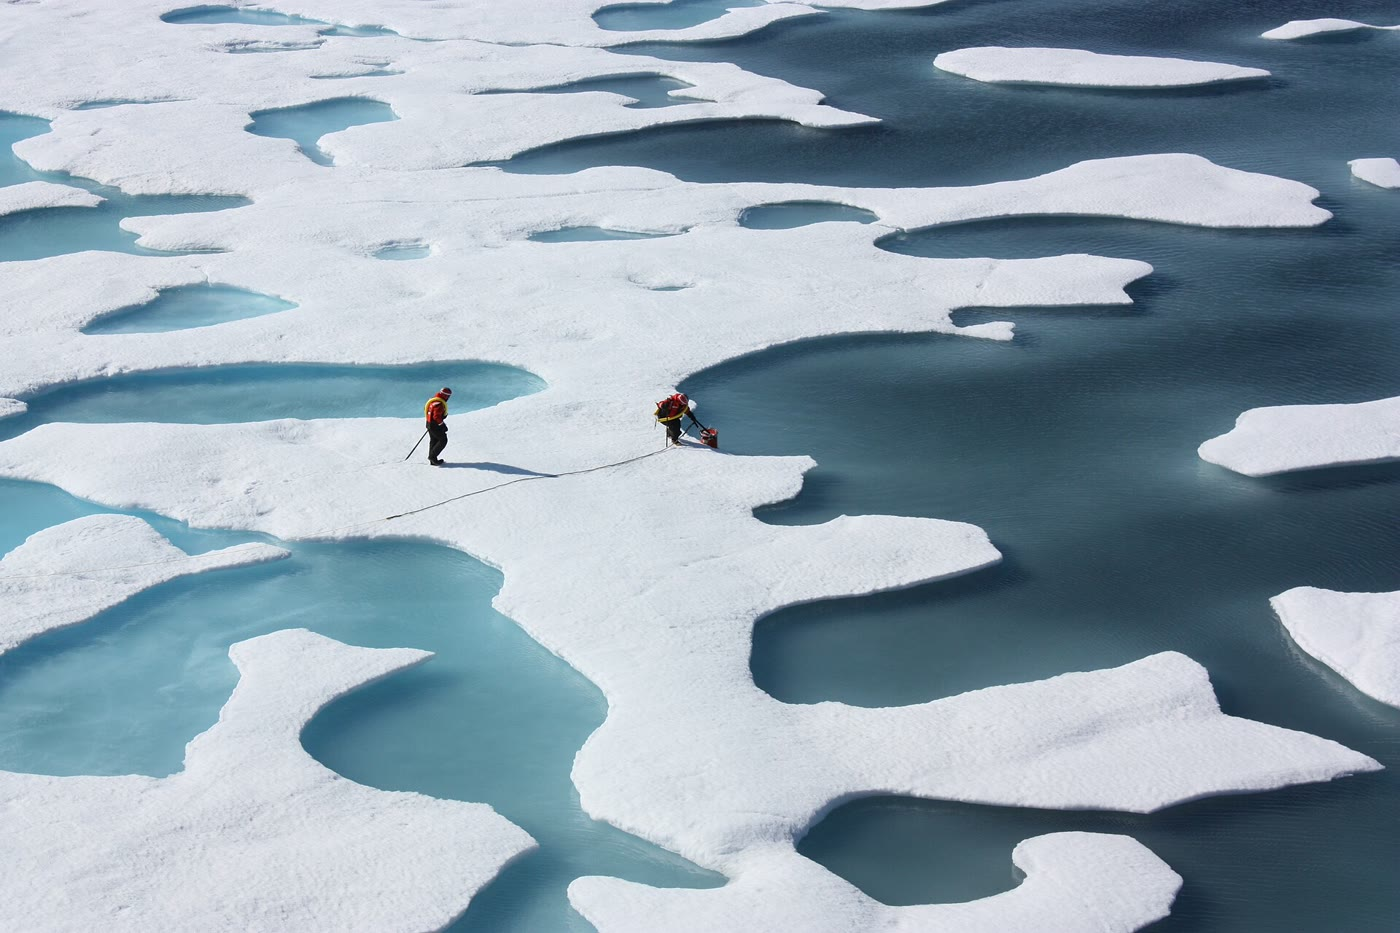
\includegraphics[width=0.78\linewidth]{images/book2/g10-nasa-melt-ponds.jpg}

{\small Hielo marino en el océano Ártico en julio, bajo un Sol que no se
pone: hielo blanco, charcas de agua de fusión sobre su superficie y el mar
oscuro y abierto entre los témpanos. Dos científicos toman muestras de las
charcas. Fotografía: NASA Goddard Space Flight Center, 2011 (dominio
público).}
\end{omfigure}

\begin{recall}
Las estaciones se deben a la inclinación del eje de la Tierra,
\qty{23.44}{\degree} respecto a la perpendicular al plano de su órbita: en
junio, el hemisferio norte se inclina hacia el Sol, que sube más alto en su
cielo y permanece más tiempo sobre el horizonte (los libros de física y el
Libro 1). La irradiancia a la distancia de la Tierra,
$S_0 = \qty{1361}{W/m^2}$, el \omterm{def:g10:earth-energy-budget:albedo}{albedo} de Bond de un planeta y su \omterm{def:g10:habitable-planet:equilibrium-temperature}{temperatura
de equilibrio} se vieron en el \cref{ch:g10:habitable-planet}. Los gases de
efecto invernadero absorben parte del infrarrojo que emite la superficie
(los libros de química). El aire caliente sube y el frío baja, lo que pone el
aire a girar en células de convección y mueve los vientos globales (Libro 1,
año 8). Las plantas, las algas y algunas bacterias fabrican azúcares a partir
de dióxido de carbono y agua con la energía de la luz: es la fotosíntesis
(los libros de biología).
\end{recall}

\section{La luz solar recibida}

Vista desde el Sol, la Tierra es un disco. Cada segundo intercepta la luz
solar que cae sobre un disco de radio $R$, su propio radio; pero esa luz se
reparte entre todos los puntos de una esfera, la mitad de los cuales están
de noche.

\begin{proposition}[Un cuarto de la constante solar]\label{prop:g10:earth-energy-budget:quarter}
Promediada sobre toda la superficie de la Tierra y sobre el día y la noche,
la potencia de la luz solar que llega a la parte alta de la atmósfera es
\[
  \frac{S_0}{4} = \frac{1361}{4} \approx \qty{340}{W/m^2}.
\]
\end{proposition}

\begin{proof}
La Tierra intercepta la luz solar que atraviesa un disco de área $\pi R^2$
perpendicular a los rayos, es decir, una potencia $S_0\,\pi R^2$. Repartida
sobre el área de la esfera, $4\pi R^2$, esto da $S_0\,\pi R^2/(4\pi R^2) =
S_0/4$ por metro cuadrado.
\end{proof}
% ledger: earth:TSI, ipcc:budget-toa

\begin{omfigure}
\begin{tikzpicture}[font=\small, >={Stealth[length=2mm]}]
  \foreach \y in {-1.2,-0.8,...,1.21}
    \draw[->, omProp!80!black] (-3.4,\y) -- (-1.75,\y);
  \node[anchor=south, font=\footnotesize, align=center] at (-2.6,1.35) {luz solar,\\$S_0$ por m$^2$};
  \draw[fill=omProp!15, draw=omProp!80!black] (-1.6,0) ellipse (0.18 and 1.3);
  \node[anchor=north, font=\footnotesize, align=center] at (-1.6,-1.4) {disco\\$\pi R^2$};
  \shade[ball color=omDef!35] (1.2,0) circle (1.3);
  \fill[black, opacity=0.35] (1.2,1.3) arc (90:-90:1.3) arc (-90:90:0.35 and 1.3);
  \draw[omDef!80!black] (1.2,0) circle (1.3);
  \draw[dashed, black!50] (1.2,-1.3) arc (-90:90:0.35 and 1.3);
  \draw[<->] (1.2,0) -- node[above, font=\footnotesize] {$R$} (2.5,0);
  \node[anchor=west, font=\footnotesize, align=left] at (2.8,0.7) {esfera $4\pi R^2$:\\mitad de día,\\mitad de noche};
  \node[anchor=west, font=\footnotesize, align=left] at (2.8,-0.75) {media:\\$S_0\pi R^2/4\pi R^2 = S_0/4$};
\end{tikzpicture}

{\small La Tierra intercepta la luz solar que cae sobre un disco de su mismo
radio, pero la reparte sobre el área cuatro veces mayor de una esfera: por
término medio, cada metro cuadrado de la parte alta de la atmósfera recibe
un cuarto de la constante solar.}
\end{omfigure}

La media oculta grandes diferencias de un lugar a otro. Un haz de luz solar
que llega al suelo de forma oblicua se reparte sobre una superficie mayor que
un haz que llega de frente.

\begin{proposition}[La luz solar sobre una superficie horizontal]\label{prop:g10:earth-energy-budget:height}
Cuando el Sol está a una altura $h$ sobre el horizonte, un metro cuadrado
horizontal de la parte alta de la atmósfera recibe la potencia $S_0 \sin h$.
\end{proposition}

\begin{proof}
Toma un haz de luz solar de sección cuadrada de \qty{1}{m^2}, que transporta
$S_0$. Sobre el suelo, su huella es un rectángulo con un lado de \qty{1}{m}
y el otro de longitud $\ell$ en la dirección de la inclinación de los rayos.
En el triángulo rectángulo que forman ese lado, el rayo y la sección del
haz, el ángulo en el suelo es $h$ y $\sin h = 1/\ell$. La potencia del haz
se reparte sobre $\ell$ metros cuadrados: $S_0/\ell = S_0 \sin h$ por metro
cuadrado.
\end{proof}

\begin{omfigure}
\begin{tikzpicture}[font=\small, >={Stealth[length=2mm]}]
  \fill[omExo!15] (-0.3,-0.5) rectangle (6.3,0);
  \draw[thick] (-0.3,0) -- (6.3,0);
  \foreach \s in {0,0.3,...,1.21}
    \draw[->, omProp!80!black] ({0.6+\s/sin(35)+3.2*cos(35)},{3.2*sin(35)}) -- ({0.6+\s/sin(35)+0.02*cos(35)},{0.02*sin(35)});
  \draw[omProp!80!black, thick] (0.6,0) -- ({0.6+1.2/sin(35)},0);
  \draw (0.6,0) ++(1.6,0) arc (0:35:1.6);
  \node[font=\footnotesize] at ({0.6+1.85*cos(17)},{1.85*sin(17)}) {$h$};
  \draw[<->] (0.6,-0.25) -- node[below, font=\footnotesize] {$\ell = 1/\sin h$} ({0.6+1.2/sin(35)},-0.25);
  \node[anchor=south west, font=\footnotesize, align=left] at (4.35,1.95) {haz de\\sección\\\qty{1}{m^2}};
\end{tikzpicture}

{\small Luz solar que llega a una altura $h$ sobre el horizonte: el mismo haz
cubre $1/\sin h$ metros cuadrados de suelo horizontal, así que cada metro
cuadrado recibe $S_0 \sin h$. Cuanto más bajo está el Sol, más débil es la
luz solar sobre el suelo.}
\end{omfigure}

La altura del Sol cambia a lo largo del día, y la duración del día cambia
con las estaciones; ambas cosas cuentan en la energía que recibe un lugar.

\begin{definition}[Insolación]\label{def:g10:earth-energy-budget:insolation}
La \emph{insolación}\index{insolacion@insolación} de un lugar es la potencia
de la luz solar que recibe un metro cuadrado horizontal en la parte alta de
la atmósfera situada sobre él. Promediada sobre las veinticuatro horas de un
día, es la \emph{insolación media diaria}; promediada sobre un año, la
\emph{insolación media anual}; ambas se miden en \unit{W/m^2}.
\end{definition}

Calcular la media diaria exige conocer la altura del Sol en cada momento del
día, lo que requiere matemáticas que van más allá de este libro; lo hizo el
ordenador que trazó las curvas de abajo. Dos casos son sencillos. En el
ecuador, en un equinoccio, el Sol sale justo por el este, pasa por el cenit a
mediodía y se pone justo por el oeste al cabo de doce horas; promediado
sobre veinticuatro horas, esto da $S_0/\pi \approx \qty{433}{W/m^2}$ (se
admite). En el Polo Norte, el Sol simplemente da vueltas por el cielo a una
altura constante, lo que aprovecha el ejemplo siguiente.

\begin{example}[El polo en junio]\label{ex:g10:earth-energy-budget:pole}
% ledger: earth:TSI, earth:obliquity (values computed in figdata/grade-10/energy_budget.py)
En el solsticio de junio, el Sol está todo el día a \qty{23.44}{\degree}
sobre el horizonte del Polo Norte. La \omterm{def:g10:earth-energy-budget:insolation}{insolación} media diaria allí es $1361
\times \sin 23.44^\circ \approx \qty{541}{W/m^2}$; en veinticuatro horas,
esto supone $541 \times 24 \approx \qty{13000}{Wh}$, \qty{13.0}{kWh} por
metro cuadrado. Ese mismo día, el ecuador recibe una media diaria de
\qty{397}{W/m^2}, es decir, \qty{9.5}{kWh} por metro cuadrado: allí el Sol
sube más alto a mediodía, pero pasa doce horas bajo el horizonte.
\end{example}

\begin{omfigure}
\begin{tikzpicture}
\begin{axis}[omrecord, width=0.92\linewidth, height=6.4cm, xmin=1, xmax=365,
  ymin=0, ymax=600, ylabel={insolación media diaria (\unit{W/m^2})},
  xtick={1,32,60,91,121,152,182,213,244,274,305,335},
  xticklabels={E,F,M,A,M,J,J,A,S,O,N,D}, xlabel={mes},
  legend style={at={(0.5,1.02)}, anchor=south, legend columns=4, font=\footnotesize, draw=none},
  tick label style={font=\small}, label style={font=\small}]
\addplot[omThm!85!black, thick] table[x=day, y=Q0] {figdata/out/grade-10-energy_budget-daily.dat};
\addlegendentry{ecuador}
\addplot[omProp!90!black, thick, densely dashed] table[x=day, y=Q30] {figdata/out/grade-10-energy_budget-daily.dat};
\addlegendentry{\qty{30}{\degree} N}
\addplot[omMeth!85!black, thick, dashdotted] table[x=day, y=Q60] {figdata/out/grade-10-energy_budget-daily.dat};
\addlegendentry{\qty{60}{\degree} N}
\addplot[omDef!85!black, thick] table[x=day, y=Q90] {figdata/out/grade-10-energy_budget-daily.dat};
\addlegendentry{Polo Norte}
\end{axis}
\end{tikzpicture}

{\small \omterm{def:g10:earth-energy-budget:insolation}{Insolación} media diaria en la parte alta de la atmósfera a lo largo
del año en cuatro latitudes del hemisferio norte (calculada para una órbita
circular, a partir de la constante solar y de la inclinación del eje). El
polo no recibe nada durante medio año, y en torno al solsticio de junio
recibe más que cualquier otro lugar.}
\end{omfigure}

\begin{remark}[Cómo leer las curvas]\label{rem:g10:earth-energy-budget:curves}
La \omterm{def:g10:earth-energy-budget:insolation}{insolación} del ecuador apenas cambia: dos máximos suaves en los
equinoccios, cuando el Sol pasa por el cenit a mediodía. Cuanto más al norte,
mayor es la oscilación entre el verano y el invierno. Más allá de
$90^\circ - 23.44^\circ = \qty{66.56}{\degree}$, el Sol permanece bajo el
horizonte en el solsticio de diciembre: es la noche polar. Desde el 10 de
mayo, aproximadamente, hasta finales de julio, el Polo Norte y la latitud
\qty{60}{\degree} N reciben ambos más que el ecuador.
\end{remark}

A lo largo de un año entero el panorama cambia: la \omterm{def:g10:earth-energy-budget:insolation}{insolación} media anual,
representada más abajo en la sección sobre excedente y déficit, baja de
\qty{416}{W/m^2} en el ecuador a \qty{172}{W/m^2} en los polos. La
abundancia estival de las regiones polares no compensa su larga noche ni la
poca altura de su Sol.

\begin{remark}[La distancia al Sol no produce las estaciones]\label{rem:g10:earth-energy-budget:distance}
% ledger: earth:peri, earth:aph, nasa:earth-perihelion-longitude (ratios computed)
La órbita de la Tierra no es exactamente una circunferencia: su distancia al
Sol varía entre \num{147.1} y \num{152.1} millones de kilómetros, alrededor
de un \qty{3}{\percent}, así que la luz solar varía alrededor de un
\qty{7}{\percent}. La Tierra está más cerca del Sol a principios de enero,
en pleno invierno boreal. Las curvas de arriba desprecian este pequeño
cambio; las estaciones se deben a la inclinación del eje, y están invertidas
en los dos hemisferios.
\end{remark}

\section{El albedo}

Parte de la luz solar que llega a la Tierra no calienta nunca nada: las
nubes, el aire, la nieve y el mar la devuelven al espacio.

\begin{definition}[Albedo]\label{def:g10:earth-energy-budget:albedo}
El \emph{albedo}\index{albedo} de una superficie es la fracción de la luz
solar que cae sobre ella y que refleja, un número entre 0 (toda la luz
absorbida) y 1 (toda reflejada). El albedo de Bond del
\cref{ch:g10:habitable-planet} es el albedo de un planeta tomado en su
conjunto.
\end{definition}

\begin{omfigure}
\begin{tikzpicture}[font=\small, x=9cm, y=0.55cm]
  \foreach \lab/\lo/\hi/\n in {nieve reciente/0.80/0.90/8, hielo marino/0.50/0.70/7,
      arena del desierto/0.40/0.40/6, Tierra entera/0.30/0.30/5, hierba verde/0.25/0.25/4,
      suelo desnudo/0.17/0.17/3, bosque de coníferas/0.08/0.15/2, océano abierto/0.06/0.06/1,
      asfalto nuevo/0.04/0.04/0} {
    \fill[omDef!45] (0,\n-0.32) rectangle (\lo,\n+0.32);
    \ifdim\hi pt>\lo pt
      \fill[omDef!18] (\lo,\n-0.32) rectangle (\hi,\n+0.32);
      \draw[omDef!80!black] (\lo,\n-0.32) rectangle (\hi,\n+0.32);
    \fi
    \draw[omDef!80!black] (0,\n-0.32) rectangle (\lo,\n+0.32);
    \node[anchor=east, font=\footnotesize] at (-0.01,\n) {\lab};
  }
  \draw (0,-0.6) -- (1,-0.6);
  \foreach \x in {0,0.2,...,1.01}
    \draw (\x,-0.6) -- (\x,-0.75) node[below, font=\footnotesize] {\pgfmathprintnumber[fixed, precision=1]{\x}};
  \node[font=\footnotesize] at (0.5,-2.0) {albedo};
\end{tikzpicture}

{\small \omterm{def:g10:earth-energy-budget:albedo}{Albedos} típicos de distintas superficies y de la Tierra en conjunto;
la parte clara de cada barra es el intervalo habitual. Datos: University of
Colorado Boulder, expedición MOSAiC; National Snow and Ice Data Center.}
\end{omfigure}
% ledger: albedo:surfaces, nsidc:albedo-ice

La nieve reciente devuelve la mayor parte de la luz que recibe; el océano
abierto, casi nada. Por eso el hielo marino de la fotografía inicial
conserva su frío durante el verano polar: la nieve que lo cubre refleja hasta
nueve décimas partes de la luz solar, mientras que el agua oscura que hay
entre los témpanos absorbe alrededor del 94 por ciento. Cuando el hielo se
funde, el agua oscura ocupa su lugar y absorbe más luz solar, lo que funde
más hielo: un bucle que se refuerza a sí mismo y que el
\cref{ch:g12:climate-change} sopesa entre las retroalimentaciones del clima.

\begin{omfigure}
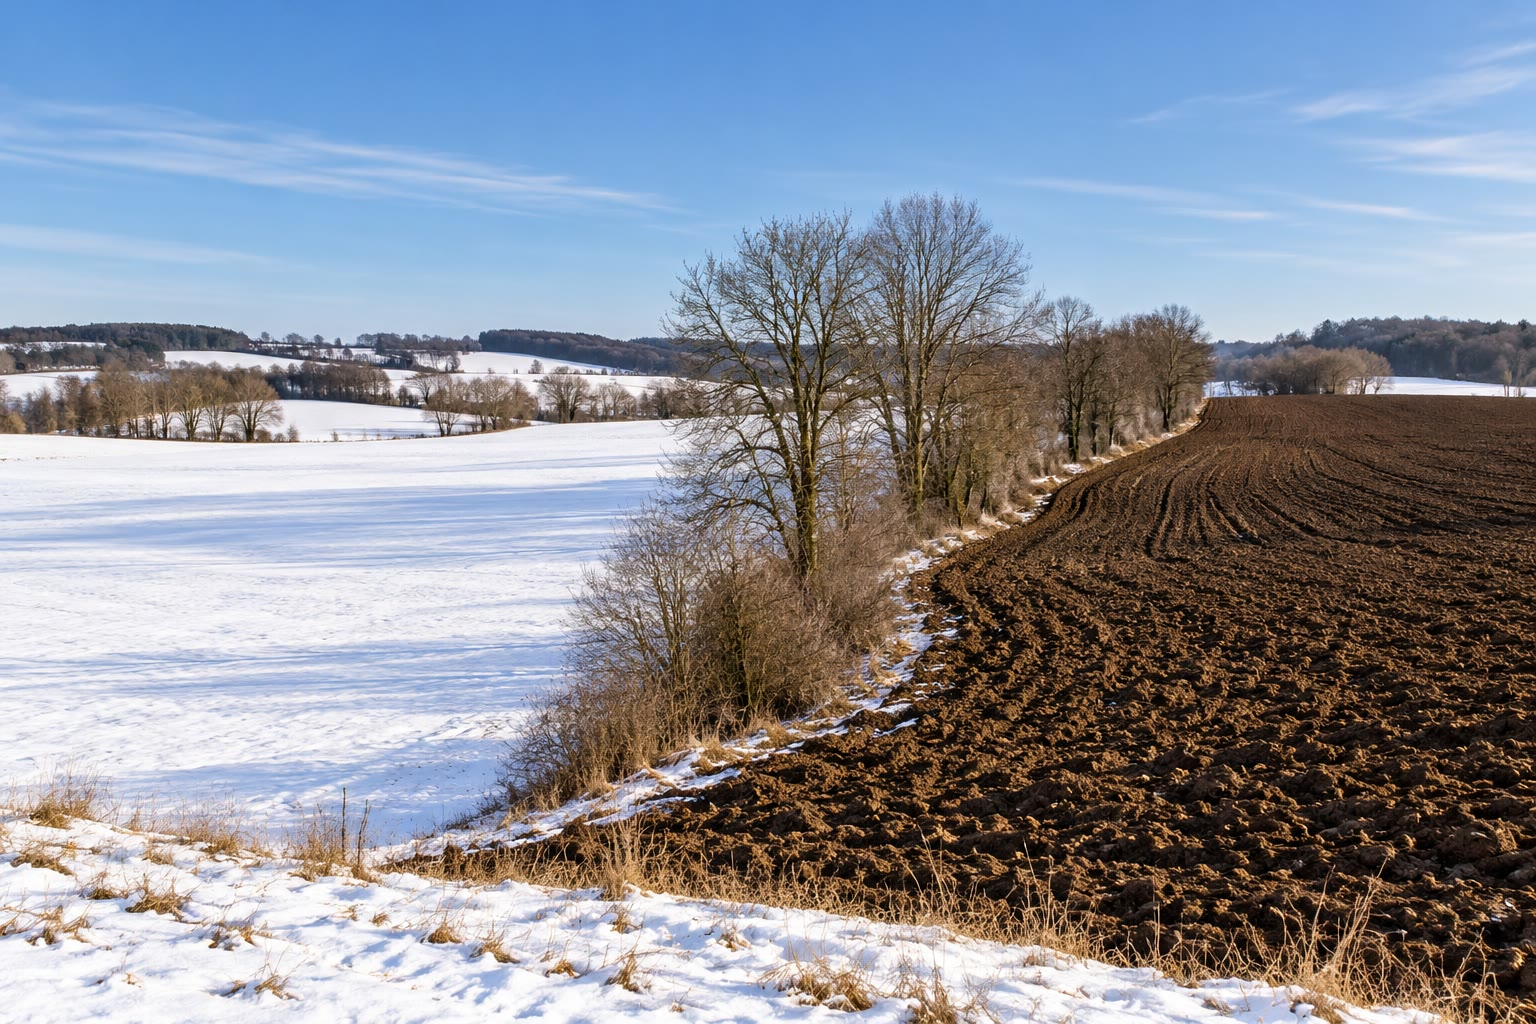
\includegraphics[width=0.7\linewidth]{images/book2/ai/g10-snow-and-ploughed-field.jpg}

{\small Una mañana de invierno tras unos días de sol: la nieve sigue sobre el
prado, pero se ha fundido en el campo arado oscuro, que absorbe mucha más luz
solar.}
\end{omfigure}

Para la Tierra en conjunto, los satélites miden directamente la luz solar
reflejada hacia el espacio: por término medio, \qty{100}{W/m^2} de los
\qty{340}{W/m^2} que llegan, un \omterm{def:g10:earth-energy-budget:albedo}{albedo} de $100/340 \approx 0.29$. Las nubes
son el principal reflector: las mismas medidas, eliminando las nubes por
cálculo, dan solo \qty{53}{W/m^2} reflejados.
% ledger: ipcc:budget-toa, ipcc:budget-clearsky, earth:albedo

\begin{example}[La luz solar que absorbe la Tierra]\label{ex:g10:earth-energy-budget:absorbed}
% ledger: earth:TSI, earth:albedo, earth:Rmean (computed in figdata/grade-10/energy_budget.py)
Con un \omterm{def:g10:earth-energy-budget:albedo}{albedo} de Bond de 0.294, cada metro cuadrado absorbe por término
medio $340
\times (1 - 0.294) \approx \qty{240}{W/m^2}$. Sobre toda la
esfera, de área
$4\pi R^2 = 4\pi \times (\qty{6.371e6}{m})^2 \approx \qty{5.10e14}{m^2}$, la
Tierra absorbe $240 \times 5.10\times10^{14} \approx \qty{1.22e17}{W}$ de luz
solar: esta potencia mueve los vientos, las corrientes oceánicas y el ciclo
del agua.
\end{example}

\section{El balance energético global}

¿Adónde van esos \qty{240}{W/m^2}? Las medidas de satélites, de
instrumentos en tierra y de barcos, combinadas con modelos de la atmósfera,
dan hoy una respuesta coherente, promediada sobre todo el globo y sobre
varios años. La evaluación científica de 2021 la resume en el diagrama de
abajo, y afirma que las componentes medias globales se conocen ahora con más
exactitud, en la parte alta de la atmósfera y en la superficie
(\emph{confianza alta}).
% ledger: ipcc:budget-confidence

\begin{definition}[Balance energético]\label{def:g10:earth-energy-budget:energy-budget}
El \emph{balance energético}\index{balance energetico@balance energético}
de un sistema ---la Tierra entera, su superficie o su atmósfera--- es la
cuenta de toda la energía que entra en él y sale de él, con cada flujo dado
como una potencia media por metro cuadrado de superficie terrestre. El
balance está \emph{equilibrado} cuando lo que entra es igual a lo que sale;
si no, el sistema gana o pierde energía y se calienta o se enfría.
\end{definition}

La superficie también pierde energía sin ninguna radiación: el agua se
evapora del mar y de las hojas, y el suelo calienta el aire que está en
contacto con él.

\begin{definition}[Calor latente; calor sensible]\label{def:g10:earth-energy-budget:latent-heat}
El \emph{calor latente}\index{calor latente} de una sustancia es la energía
que absorbe cuando cambia de estado sin cambiar de temperatura ---al
fundirse o al evaporarse--- y que devuelve cuando vuelve a cambiar. Para el
agua que se evapora a \qty{15}{\degreeCelsius} es de unos \qty{2.47}{MJ}
por kilogramo. En el \omterm{def:g10:earth-energy-budget:energy-budget}{balance energético}, el \emph{flujo de calor latente} es
la energía que la evaporación toma de la superficie y que el vapor de agua
libera en el aire, allí donde se condensa en nubes. El flujo de \emph{calor
sensible}\index{calor sensible} es la energía que la superficie cede al aire
en contacto con ella, calentándolo, y que el aire ascendente transporta hacia
arriba.
\end{definition}
% ledger: nist:water-latent

\begin{omfigure}
\begin{tikzpicture}[font=\footnotesize, >={Stealth[length=2.2mm, width=2mm]}, line width=1.4pt]
  % layers
  \fill[omDef!8] (0,0.5) rectangle (12.8,4.5);
  \fill[omExo!35] (0,0) rectangle (12.8,0.5);
  \draw[thin, black!60] (0,0.5) -- (12.8,0.5);
  \draw[thin, black!60, dashed] (0,4.5) -- (12.8,4.5);
  \node[anchor=east, black!70, align=right] at (-0.1,5.4) {espacio};
  \node[anchor=east, black!70, align=right] at (-0.1,4.5) {parte alta de\\la atmósfera};
  \node[anchor=east, black!70, align=right] at (-0.1,2.5) {atmósfera};
  \node[anchor=east, black!70, align=right] at (-0.1,0.25) {superficie};
  \pic[scale=0.7, transform shape] at (4.3,3.0) {puffycloud};
  \pic[scale=0.7, transform shape] at (6.2,3.0) {puffycloud};
  % sunlight
  \draw[->, omProp!90!black] (1.0,6.1) -- (1.0,0.52);
  \draw[->, omProp!90!black] (1.0,3.0) -- (1.6,3.0);
  \node[anchor=west, align=left] at (1.65,3.0) {80 absorbidos\\por el aire};
  \node[anchor=west] at (1.05,1.3) {185};
  \draw[->, omProp!55] (4.3,3.7) -- (4.3,6.1);
  \node[anchor=east] at (4.25,5.0) {75};
  \draw[->, omProp!55] (5.25,0.52) -- (5.25,6.1);
  \node[anchor=west] at (5.3,1.2) {25};
  % heat
  \draw[->, omMeth!80!black] (6.2,0.52) -- (6.2,2.95);
  \draw[->, omMeth!80!black] (7.8,0.52) -- (7.8,2.0);
  % infrared
  \draw[->, omThm!80!black] (9.2,0.52) -- (9.2,4.0);
  \draw[->, omThm!80!black] (10.7,3.4) -- (10.7,6.1);
  \draw[->, omThm!50] (12.1,4.0) -- (12.1,0.52);
  % words above the top of the atmosphere
  \node[anchor=south, align=center] at (1.0,6.15) {340\\entrantes};
  \node[anchor=south, align=center] at (4.78,6.15) {100\\reflejados};
  \node[anchor=south, align=center] at (7.7,5.0) {desequilibrio:\\$+0.7$ absorbidos};
  \node[anchor=south, align=center] at (10.7,6.15) {239 infrarrojo\\al espacio};
  % words below the surface
  \node[anchor=north, align=center] at (1.0,-0.05) {160\\absorbidos};
  \node[anchor=north, align=center] at (6.2,-0.05) {82\\calor\\latente};
  \node[anchor=north, align=center] at (7.8,-0.05) {21\\calor\\sensible};
  \node[anchor=north, align=center] at (9.4,-0.05) {398\\emitidos};
  \node[anchor=north, align=center] at (12.1,-0.05) {342\\radiación\\de retorno};
\end{tikzpicture}

{\small El \omterm{def:g10:earth-energy-budget:energy-budget}{balance energético} medio global de la Tierra a principios del
siglo XXI, en \unit{W/m^2} promediados sobre toda la superficie. Naranja: luz
solar; verde: calor transportado por la evaporación y por el aire caliente;
rojo: infrarrojo. De los 100 reflejados, 25 proceden de la superficie y 75 de
las nubes, del aire y de su polvo. El infrarrojo hacia el espacio incluye la
parte de la emisión de la superficie que escapa directamente a través del
aire. Datos: IPCC, Sexto Informe de Evaluación, Grupo de Trabajo~I,
Figura~7.2.}
\end{omfigure}
% ledger: ipcc:budget-toa, ipcc:budget-surface

\begin{method}[Leer un diagrama de balance energético]\label{met:g10:earth-energy-budget:reading}
\begin{enumerate}
  \item Elige el sistema: la Tierra entera (una línea por encima de la
        atmósfera), la superficie o la atmósfera (la capa entre ambas).
  \item Haz la lista de las flechas que entran en él y súmalas; haz la lista
        de las flechas que salen de él y súmalas.
  \item Compara las dos sumas. Si son iguales, salvo por el redondeo de los
        números, el sistema está en equilibrio; la diferencia es lo que gana
        (o pierde) cada segundo por metro cuadrado.
\end{enumerate}
\end{method}

\begin{proposition}[El balance cuadra]\label{prop:g10:earth-energy-budget:balance}
Salvo por el redondeo de las cifras, el balance del diagrama de arriba está
equilibrado para la Tierra en conjunto, para la superficie y para la
atmósfera, aparte de un pequeño excedente de unos \qty{0.7}{W/m^2} que la
Tierra absorbe y no devuelve.
\end{proposition}

\begin{proof}
\emph{Tierra entera:} entra 340; sale $100 + 239 = 339$. \emph{Superficie:}
entra $160 + 342 = 502$; sale $82 + 21 + 398 = 501$. En ambos casos el
excedente, de alrededor de 1, es el desequilibrio de 0.7 redondeado.
\emph{Atmósfera:} llama $W$ a la parte del infrarrojo de la superficie que
escapa a través del aire hacia el espacio. El aire recibe
$80 + 82 + 21 + (398 - W) = 581 - W$ y emite $342$ hacia abajo y
$239 - W$ hacia arriba, $581 - W$ en total: equilibrado, sea cual sea $W$.
\end{proof}
% ledger: ipcc:budget-toa, ipcc:budget-surface (closures checked in figdata/grade-10/energy_budget.py)

El diagrama muestra también el efecto invernadero en acción. La superficie
recibe del aire, en forma de infrarrojo, \qty{342}{W/m^2}: más del doble de
la luz solar que absorbe, \qty{160}{W/m^2}. Por eso puede emitir
\qty{398}{W/m^2}, la emisión de un cuerpo a unos \qty{15}{\degreeCelsius},
mientras que la Tierra solo envía \qty{239}{W/m^2} al espacio. Los libros de
física construyen el modelo que relaciona estos números con la temperatura;
este libro usa los flujos medidos.

\begin{example}[Un metro de agua al año]\label{ex:g10:earth-energy-budget:evaporation}
% ledger: ipcc:budget-surface, nist:water-latent (computed in figdata/grade-10/energy_budget.py)
El flujo de \omterm{def:g10:earth-energy-budget:latent-heat}{calor latente}, \qty{82}{W/m^2}, evapora cada segundo
$82/2.47\times
10^6 \approx \qty{3.3e-5}{kg}$ de agua por metro cuadrado. En
un año, $3.16\times10^7$ segundos, esto suma unos \qty{1050}{kg}, una capa de
agua de \qty{1.05}{m} de espesor sobre toda la Tierra. El aire solo contiene
un poco de agua a la vez, así que prácticamente toda ella vuelve a caer como
lluvia y nieve: el flujo de \omterm{def:g10:earth-energy-budget:latent-heat}{calor latente} y la precipitación anual del
planeta son dos caras del mismo ciclo del agua.
\end{example}

\begin{remark}[El desequilibrio]\label{rem:g10:earth-energy-budget:imbalance}
% ledger: ipcc:budget-toa, ipcc:heating
El excedente de \qty{0.7}{W/m^2} parece minúsculo al lado de flujos de
cientos de vatios, pero sobre toda la Tierra supone
$0.7 \times 5.10\times10^{14} \approx
\qty{3.6e14}{W}$, almacenados sobre
todo en el océano, que se calienta. No es una constante natural: ha crecido
en las últimas décadas, como explica el \cref{ch:g12:climate-change}.
\end{remark}

\section{Excedente y déficit}

El balance cuadra para la Tierra en conjunto, pero no en cada latitud.

\begin{omfigure}
\begin{tikzpicture}
\begin{axis}[omrecord, width=0.86\linewidth, height=5.6cm, xmin=0, xmax=90,
  ymin=0, ymax=450, xlabel={latitud (\unit{\degree})},
  ylabel={insolación media anual (\unit{W/m^2})}, xtick={0,15,...,90},
  tick label style={font=\small}, label style={font=\small}]
\addplot[omThm!85!black, thick] table[x=lat, y=Qann] {figdata/out/grade-10-energy_budget-annual.dat};
\addplot[omDef!80!black, dashed, domain=0:90] {340.25};
\node[anchor=south west, font=\footnotesize, omDef!80!black] at (axis cs:2,343) {media global, 340};
\node[anchor=south west, font=\footnotesize, omThm!85!black] at (axis cs:62,232) {media anual};
\end{axis}
\end{tikzpicture}

{\small \omterm{def:g10:earth-energy-budget:insolation}{Insolación} media anual en la parte alta de la atmósfera en función
de la latitud (la misma en ambos hemisferios; calculada a partir de la
constante solar y de la inclinación del eje). Entre el ecuador y unos
\qty{37}{\degree} supera la media global; más hacia los polos queda por
debajo.}
\end{omfigure}

Los trópicos absorben mucha más luz solar que las regiones polares, y su
bajo \omterm{def:g10:earth-energy-budget:albedo}{albedo} agranda la diferencia. El infrarrojo que envían al espacio
también es mayor, porque están más calientes, pero varía mucho menos con la
latitud. En consecuencia, las regiones próximas al ecuador absorben por
término medio unos \qty{200}{W/m^2} más de lo que reflejan y radian, y las
regiones cercanas a los polos radian unos \qty{200}{W/m^2} más de lo que
absorben.
% ledger: nasaeo:surplus

\begin{definition}[Transporte de calor hacia los polos]\label{def:g10:earth-energy-budget:heat-transport}
El \emph{transporte de calor hacia los polos}\index{transporte de calor hacia los polos}
es el flujo de energía que los movimientos de la atmósfera y del océano
llevan de los trópicos hacia los polos. Se mide, a través de un círculo de
latitud, en petavatios (\qty{1}{PW} = \qty{e15}{W}).
\end{definition}

Sin él, los trópicos se calentarían y los polos se enfriarían hasta que cada
latitud equilibrara su propio balance. La atmósfera hace la mayor parte del
transporte: aire caliente que se desplaza hacia los polos y aire frío que
vuelve hacia el ecuador, y vapor de agua que libera su \omterm{def:g10:earth-energy-budget:latent-heat}{calor latente} lejos
de donde se evaporó. Las corrientes oceánicas transportan el resto. Las
estimaciones a partir de medidas sitúan el transporte atmosférico hacia los
polos en un máximo de unos \qty{5.0}{PW} cerca de \qty{43}{\degree} N, con
valores parecidos cerca de \qty{40}{\degree} S; el océano transporta más que
la atmósfera solo cerca del ecuador, entre \qty{0}{\degree} y
\qty{17}{\degree} N, y a \qty{35}{\degree} N, donde el transporte total es
máximo, la atmósfera lleva el \qty{78}{\percent}. El total es máximo allí
porque \qty{35}{\degree} es, más o menos, donde el excedente da paso al
déficit: hacia el ecuador, el transporte sigue recogiendo el excedente de
cada latitud que atraviesa; hacia los polos, cada latitud se nutre de él.
% ledger: trenberth:transport

\begin{omfigure}
\begin{tikzpicture}[font=\footnotesize, >={Stealth[length=2mm]}]
  \def\R{2.4}
  \begin{scope}
    \clip (0,0) circle (\R);
    \fill[omThm!22] (-\R,{-\R*sin(35)}) rectangle (\R,{\R*sin(35)});
    \fill[omDef!22] (-\R,{\R*sin(35)}) rectangle (\R,\R);
    \fill[omDef!22] (-\R,-\R) rectangle (\R,{-\R*sin(35)});
  \end{scope}
  \draw[thick] (0,0) circle (\R);
  \draw[black!50] (-\R,0) -- (\R,0);
  \foreach \s in {1,-1} \draw[black!40, dashed] ({-\R*cos(35)},{\s*\R*sin(35)}) -- ({\R*cos(35)},{\s*\R*sin(35)});
  \node at (0,0.45) {excedente};
  \node at (0,1.95) {déficit};
  \node at (0,-1.95) {déficit};
  \node[anchor=west, black!60] at (\R+0.05,0) {ecuador};
  \node[anchor=west, black!60] at ({\R*cos(35)+0.05},{\R*sin(35)}) {\qty{35}{\degree} N};
  \node[anchor=west, black!60] at ({\R*cos(35)+0.05},{-\R*sin(35)}) {\qty{35}{\degree} S};
  \foreach \s in {1,-1} {
    \draw[->, very thick, omProp!90!black] ({-(\R+0.35)*cos(10)},{\s*(\R+0.35)*sin(10)}) arc ({180-10*\s}:{180-70*\s}:{\R+0.35});
    \draw[->, thick, omMeth!80!black] ({-(\R-0.45)*cos(8)},{\s*(\R-0.45)*sin(8)}) arc ({180-8*\s}:{180-55*\s}:{\R-0.45});
  }
  \node[anchor=east, omProp!90!black, align=right] at (-\R-0.75,1.6) {atmósfera};
  \node[anchor=east, omProp!90!black, align=right] at (-\R-0.75,-1.6) {atmósfera};
  \node[omMeth!80!black] at (-1.25,0.62) {océano};
  \node[omMeth!80!black] at (-1.25,-0.62) {océano};
\end{tikzpicture}

{\small Entre unos \qty{35}{\degree} S y \qty{35}{\degree} N, la Tierra
absorbe más energía de la que radia; más allá de estas latitudes, radia más
de la que absorbe. La atmósfera (naranja) y el océano (verde) transportan el
excedente hacia los polos. Esquema: el grosor de las flechas no está a
escala.}
\end{omfigure}

Este transporte es el motor del tiempo atmosférico. Las células de
convección y los vientos globales del Libro 1, las tormentas del
\cref{ch:g10:storms-and-cyclones} y las grandes corrientes oceánicas del
\cref{ch:g10:layered-ocean} trasladan calor de donde el Sol da demasiado a
donde da demasiado poco.

\section{Adónde va la energía}

Casi toda la energía de la luz solar que absorbe la Tierra acaba
convertida en calor: calienta el suelo, el mar y el aire, evapora agua, mueve
los vientos y las corrientes, y vuelve a salir en forma de luz infrarroja.
Una parte diminuta sigue otro camino: la fotosíntesis la almacena en los
enlaces químicos de los azúcares, y de ahí en toda la materia viva del
planeta.

\begin{example}[La parte de la fotosíntesis]\label{ex:g10:earth-energy-budget:photosynthesis}
% ledger: field:npp, nist:glucose-combustion, earth:Rmean (computed in figdata/grade-10/energy_budget.py)
Las plantas de tierra firme y las algas del mar almacenan, después de cubrir
sus propias necesidades, unos \num{105}~mil millones de toneladas de carbono
en materia viva nueva cada año, aproximadamente la mitad en tierra y la mitad
en el océano: los ecólogos lo llaman la producción primaria neta del
planeta. Quemar un mol de glucosa, \ce{C6H12O6}, que contiene seis moles de
carbono, \qty{72}{g}, libera \qty{2805}{kJ}: unos \qty{38.9}{kJ} por gramo de
carbono. La energía almacenada cada año es
$1.049\times10^{17}\,\unit{g} \times \qty{38.9e3}{J/g} \approx
\qty{4.1e21}{J}$, una potencia de $4.1\times10^{21}/3.16\times10^{7} \approx
\qty{1.3e14}{W}$. Comparada con los \qty{1.22e17}{W} de luz solar que absorbe
la Tierra, es alrededor de un \qty{0.1}{\percent}.
\end{example}

\begin{remark}[Una parte pequeña, un papel grande]\label{rem:g10:earth-energy-budget:life}
Una milésima parte de la luz solar absorbida alimenta casi toda la vida de la
Tierra, y los restos de plantas y algas enterrados durante cientos de
millones de años forman el carbón, el petróleo y el gas natural
(\cref{ch:g11:fossil-fuel-geology}). El resto de la luz solar ---más del 99.9
por ciento--- mantiene caliente el planeta y en movimiento su aire, su agua y
su tiempo atmosférico.
\end{remark}

\section{Ejercicios}

\begin{exercise}[$\star$]\label{exo:g10:earth-energy-budget:1}
Define la \omterm{def:g10:earth-energy-budget:insolation}{insolación} de un lugar y el \omterm{def:g10:earth-energy-budget:albedo}{albedo} de una superficie. ¿Qué refleja
una fracción mayor de la luz solar, la nieve reciente o el océano abierto?
\end{exercise}

\begin{exercise}[$\star$]\label{exo:g10:earth-energy-budget:2}
Con el diagrama del \omterm{def:g10:earth-energy-budget:energy-budget}{balance energético} de este capítulo, da en porcentaje de
los \qty{340}{W/m^2} que llegan a la parte alta de la atmósfera la parte
reflejada hacia el espacio, la parte absorbida por el aire y la parte
absorbida por la superficie.
\end{exercise}

\begin{exercise}[$\star$]\label{exo:g10:earth-energy-budget:3}
Un sol de verano aporta \qty{800}{W/m^2} al suelo. ¿Qué potencia absorbe un
metro cuadrado cubierto de asfalto nuevo (\omterm{def:g10:earth-energy-budget:albedo}{albedo} 0.04), y uno cubierto de
nieve reciente (\omterm{def:g10:earth-energy-budget:albedo}{albedo} 0.85)?
\end{exercise}

\begin{exercise}[$\star$]\label{exo:g10:earth-energy-budget:4}
¿Qué se lleva más energía de la superficie terrestre, la evaporación o el
calentamiento del aire en contacto con el suelo? Describe en dos frases cómo
la energía que la evaporación toma del mar llega al aire de las capas altas.
\end{exercise}

\begin{exercise}[$\star$]\label{exo:g10:earth-energy-budget:5}
Explica por qué la \omterm{def:g10:earth-energy-budget:insolation}{insolación} media diaria es nula en el Polo Norte en
diciembre, y da la latitud a partir de la cual ocurre esto en el solsticio
de diciembre.
\end{exercise}

\begin{exercise}[$\star\star$]\label{exo:g10:earth-energy-budget:6}
Con la \cref{prop:g10:earth-energy-budget:height}, calcula la potencia que
recibe un metro cuadrado horizontal en la parte alta de la atmósfera cuando
el Sol está a \qty{90}{\degree}, \qty{30}{\degree} y \qty{10}{\degree} sobre
el horizonte. ¿A qué altura del Sol recibe el metro cuadrado la mitad de
$S_0$?
\end{exercise}

\begin{exercise}[$\star\star$]\label{exo:g10:earth-energy-budget:7}
Siguiendo el \cref{met:g10:earth-energy-budget:reading}, comprueba el
balance de la luz solar sola: de los \qty{340}{W/m^2} que llegan, ¿cuánto se
refleja, cuánto absorbe el aire y cuánto absorbe la superficie? ¿Suman las
tres cantidades 340? Comprueba también que la luz solar que llega a la
superficie, \qty{185}{W/m^2}, se refleja o se absorbe allí.
\end{exercise}

\begin{exercise}[$\star\star$]\label{exo:g10:earth-energy-budget:8}
Con el radio medio de la Tierra, \qty{6371}{km}, calcula el área del disco
que intercepta la luz solar y la potencia que intercepta, y después el área
de la esfera. Deduce la potencia media por metro cuadrado de la esfera.
\end{exercise}

\begin{exercise}[$\star\star$]\label{exo:g10:earth-energy-budget:9}
El excedente de la Tierra es de \qty{0.7}{W/m^2} sobre una superficie de
\qty{5.10e14}{m^2}. ¿Cuánta energía, en julios, gana la Tierra en un año de
$3.16\times10^7$ segundos?
\end{exercise}

\begin{exercise}[$\star\star$]\label{exo:g10:earth-energy-budget:10}
Si se eliminaran las nubes por cálculo, la Tierra reflejaría
\qty{53}{W/m^2} en lugar de \qty{100}{W/m^2}, y enviaría al espacio
\qty{267}{W/m^2} de infrarrojo en lugar de \qty{239}{W/m^2}. ¿En cuánto
cambian las nubes la luz solar absorbida, y el infrarrojo perdido? En el
balance final, ¿calientan o enfrían la Tierra las nubes?
\end{exercise}

\begin{exercise}[$\star\star$]\label{exo:g10:earth-energy-budget:11}
Lee las curvas de \omterm{def:g10:earth-energy-budget:insolation}{insolación} media diaria de este capítulo. ¿En qué meses es
la \omterm{def:g10:earth-energy-budget:insolation}{insolación} media diaria en el Polo Norte mayor que en el ecuador? ¿Por qué
muestra la curva del ecuador dos máximos y no uno?
\end{exercise}

\begin{exercise}[$\star\star\star$]\label{exo:g10:earth-energy-budget:12}
El \omterm{def:g10:earth-energy-budget:latent-heat}{calor latente} de evaporación del agua es de \qty{2.47}{MJ/kg} y el flujo
de \omterm{def:g10:earth-energy-budget:latent-heat}{calor latente}, de \qty{82}{W/m^2}. Calcula el espesor de agua, en
milímetros, que se evapora cada día del metro cuadrado medio de la Tierra, y
en metros cada año (un litro de agua extendido sobre un metro cuadrado forma
una capa de \qty{1}{mm} de espesor).
\end{exercise}

\begin{exercise}[$\star\star\star$]\label{exo:g10:earth-energy-budget:13}
En el Polo Norte, el Sol da vueltas por el cielo a una altura igual a su
declinación $\delta$, así que la \omterm{def:g10:earth-energy-budget:insolation}{insolación} media diaria allí es $S_0 \sin
\delta$. Halla la declinación para la que el polo recibe, por término medio
a lo largo del día, tanto como el ecuador en un equinoccio, $S_0/\pi$. La
declinación cumple $\sin\delta = \sin 23.44^\circ \times \sin\lambda$, donde
el ángulo $\lambda$ crece de manera uniforme \qty{360}{\degree} en un año,
desde \qty{0}{\degree} en el equinoccio de marzo (\qty{90}{\degree} en el
solsticio de junio). ¿Durante cuántos días al año, aproximadamente, recibe
el polo más de $S_0/\pi$?
\end{exercise}

\begin{exercise}[$\star\star\star$]\label{exo:g10:earth-energy-budget:14}
Supón que en verano se funde una superficie de \qty{1e12}{m^2} de hielo
marino (\omterm{def:g10:earth-energy-budget:albedo}{albedo} 0.6) y que la sustituye océano abierto (\omterm{def:g10:earth-energy-budget:albedo}{albedo} 0.06), bajo una
luz solar de \qty{300}{W/m^2} de media en la superficie. Calcula la potencia
absorbida de más. Compárala con la potencia almacenada por toda la
fotosíntesis de la Tierra, \qty{1.3e14}{W}, y explica por qué este cambio de
superficies se refuerza a sí mismo.
\end{exercise}

\begin{exercise}[$\star\star\star$]\label{exo:g10:earth-energy-budget:15}
La distancia de la Tierra al Sol es de \num{147.1} millones de kilómetros en
su punto más cercano y de \num{152.1} millones en el más lejano, con una
media de \num{149.6} millones, a la que $S_0 = \qty{1361}{W/m^2}$. Calcula la
irradiancia solar en los dos extremos. La diferencia ronda los
\qty{90}{W/m^2}; a \qty{60}{\degree} N, la \omterm{def:g10:earth-energy-budget:insolation}{insolación} media diaria es de unos
\qty{490}{W/m^2} en junio y de \qty{24}{W/m^2} en diciembre. Explica por qué
la distancia no puede ser la causa de las estaciones.
\end{exercise}

\section{Problema: siguiendo un rayo de sol}

\begin{problem}[{Problema de fin de semana --- de la luz solar que llega a la
Tierra a la parte que almacena la vida}]
\label{pb:g10:earth-energy-budget:1}
% ledger: earth:TSI, earth:Rmean, ipcc:budget-toa, ipcc:budget-surface, ipcc:budget-clearsky, nist:water-latent, field:npp, nist:glucose-combustion (all results computed in figdata/grade-10/energy_budget.py or from the rounded data below)
Usa $S_0 = \qty{1361}{W/m^2}$, el radio de la Tierra $R = \qty{6371}{km}$,
$\sigma = \qty{5.67e-8}{W.m^{-2}.K^{-4}}$, un año de $3.156\times10^7$
segundos, los flujos del diagrama del \omterm{def:g10:earth-energy-budget:energy-budget}{balance energético}, un \omterm{def:g10:earth-energy-budget:latent-heat}{calor latente}
de evaporación de \qty{2.47}{MJ/kg}, una producción primaria neta global de
\num{104.9}~mil millones de toneladas de carbono al año, y los
\qty{2805}{kJ} que libera la combustión de un mol de glucosa
(\qty{72.07}{g} de carbono).

\medskip
\noindent\textbf{Parte I --- La geometría de la luz solar.}
\begin{enumerate}
  \item Calcula el área del disco que intercepta la luz solar, $\pi R^2$, en
        metros cuadrados.
  \item Calcula la potencia de la luz solar que intercepta.
  \item Calcula el área de la superficie terrestre, $4\pi R^2$.
  \item Deduce la potencia media que llega por metro cuadrado a la parte alta
        de la atmósfera.
  \item En un equinoccio, a mediodía, el Sol está en el cenit sobre el
        ecuador y a \qty{30}{\degree} sobre el horizonte a \qty{60}{\degree} N.
        ¿Qué recibe un metro cuadrado horizontal en cada lugar?
\end{enumerate}

\medskip
\noindent\textbf{Parte II --- El albedo.}
\begin{enumerate}[resume]
  \item A partir de los \qty{100}{W/m^2} reflejados, calcula el \omterm{def:g10:earth-energy-budget:albedo}{albedo} de la
        Tierra.
  \item Calcula la potencia absorbida por metro cuadrado y por toda la
        Tierra.
  \item Sin nubes, se reflejarían \qty{53}{W/m^2}. ¿Cuál sería el \omterm{def:g10:earth-energy-budget:albedo}{albedo}?
        ¿Por qué factor lo aumentan las nubes?
  \item Calcula la \omterm{def:g10:habitable-planet:equilibrium-temperature}{temperatura de equilibrio} que corresponde a la potencia
        absorbida de la pregunta 7 (\cref{ch:g10:habitable-planet}) y
        compárala con los \qty{288}{K} de la superficie.
\end{enumerate}

\medskip
\noindent\textbf{Parte III --- La superficie.}
\begin{enumerate}[resume]
  \item Suma los flujos de energía que entran en la superficie.
  \item Suma los que salen de ella y compáralos.
  \item ¿Cuántas veces mayor que la luz solar absorbida por la superficie es
        el infrarrojo que recibe del aire? ¿Qué muestra esto?
  \item Calcula la masa de agua evaporada de un metro cuadrado en un año, y
        el espesor de la capa que forma.
  \item Calcula la potencia total del desequilibrio, \qty{0.7}{W/m^2}, sobre
        toda la Tierra.
\end{enumerate}

\medskip
\noindent\textbf{Parte IV --- La parte de la vida.}
\begin{enumerate}[resume]
  \item Calcula la energía almacenada por gramo de carbono fijado en la
        glucosa.
  \item Calcula la energía almacenada en un año por la producción primaria
        neta.
  \item Conviértela en una potencia.
  \item Exprésala por metro cuadrado de superficie terrestre.
  \item Compárala con el desequilibrio de la pregunta 14.
  \item ¿Qué parte de la luz solar absorbida por la Tierra (pregunta 7)
        almacena la fotosíntesis?
\end{enumerate}
\end{problem}
